\documentclass[conference]{IEEEtran}

\usepackage[utf8]{inputenc}
\usepackage[T1]{fontenc}
\usepackage{amsmath,amssymb,amsfonts}
\usepackage{graphicx}
\usepackage{booktabs}
\usepackage{cite}
\usepackage{xcolor}
\usepackage{hyperref}
\usepackage{listings}
\usepackage{float}
\usepackage{subcaption}
\usepackage{caption}
\usepackage{multirow}

% -------------------------------------------
% HEADER (Top-left: "ECE..." , Top-right: page #)
% -------------------------------------------
\makeatletter
\def\ps@headings{%
  \def\@oddhead{\footnotesize
    ECE, NTUA - Pattern Recognition Semester Project, February 2025%
    \hfill \thepage}%
  \def\@evenhead{\@oddhead}%
  \def\@oddfoot{}%
  \def\@evenfoot{}%
}
\makeatother
\pagestyle{headings}  % Activate the custom heading style

% -------------------------------------------
% TITLE & AUTHOR
% -------------------------------------------
\title{\Huge Kolmogorov-Arnold Networks/Transformers}

\author{
    \IEEEauthorblockN{
        Dimitrios Georgoulopoulos, \textbf{03120008},\,
        Ioannis Karaparisis, \textbf{03120866},\,
        Ioakeim El-Hattab Bistrogiannis, \textbf{03120058},\\
        Panagiotis-Alexios Spanakis, \textbf{03400274},\,
        Gregory Trakas, \textbf{03400274}
    }
}

\begin{document}

% Create the title and the abstract in the first page’s two-column format:
\maketitle

\begin{abstract}

\end{abstract}

\begin{IEEEkeywords}
\end{IEEEkeywords}

\section{Introduction}

\section{Related Work}

\subsection{Kolmogorov-Arnold Networks (KANs)}

The Kolmogorov–Arnold representation theorem states, in simplified form, that
any continuous, real‐valued function of several variables can be represented as
a superposition of continuous univariate functions combined through addition.
This insight inspires Kolmogorov–Arnold Networks (KANs), which aim to
approximate complex functions by leveraging learnable univariate activation
functions along the network’s edges \cite{kans}.

In traditional multilayer perceptrons (MLPs), learning is achieved through a
sequence of linear transformations followed by fixed pointwise nonlinearities
(e.g., ReLU). KANs, by contrast, integrate flexible, spline‐based activation
functions into each edge of the network. These splines can be refined by
increasing the number of knots, thus enhancing the function approximation in an
adaptive manner. For example, the original Kolmogorov–Arnold representation
naturally corresponds to a 2-layer KAN with a shape of \([n,\,2n+1,\,1]\),
where all operations are differentiable and the network can be trained via back
propagation.

A critical aspect of KAN implementation is the use of \emph{residual activation
    functions}. In practice, the activation function \(\phi(x)\) is defined as the
sum of a fixed basis function and a trainable spline component:
\[
    \phi(x) = w_b\,b(x) + w_s\,\text{spline}(x).
\]
Here, the basis function is typically chosen as the SiLU (sigmoid-weighted
linear unit),
\[
    b(x) = \text{silu}(x) = \frac{x}{1+e^{-x}},
\]
and the spline function is expressed as a linear combination of B-spline basis
functions:
\[
    \text{spline}(x) = \sum_i c_i\,B_i(x),
\]
with the coefficients \(c_i\) being learned during training. The trainable
factors \(w_b\) and \(w_s\) further control the overall magnitude of the
activation function.

Proper initialization is essential for stable training. Typically, the spline
component is initialized near zero (using a small variance, e.g.,
\(\sigma=0.1\) for the B-spline coefficients), while \(w_b\) is initialized
following standard methods such as Xavier initialization. Moreover, since
B-splines are defined on bounded intervals yet activation values may exceed
these bounds during training, the spline grids are updated dynamically based on
the input activations to maintain approximation accuracy.

Although, in theory, a KAN layer for a network of depth \(L\) and constant
width \(N\) (with splines of order \(k\) defined over \(G\) intervals) requires
\(\mathcal{O}(N^{2L}(G+k))\) parameters, KANs are typically designed with much
smaller widths \(N\) than conventional MLPs. This design choice not only
reduces the overall parameter count but also contributes to better
generalization, as demonstrated in the original works.

In summary, Kolmogorov–Arnold Networks offer a principled and efficient
alternative to traditional MLPs by directly learning an adaptive, spline-based
decomposition of complex functions. This unified treatment of linear
transformations and nonlinear activations yields lower test errors and improved
interpretability, especially when modeling smooth or piecewise-smooth target
functions.

\section{Reproduction Results for Toy and Special Functions}

In our reproduction study, we closely followed the experimental setup and
evaluation criteria described in the original KAN work. Our experiments were
divided into two parts: one focusing on toy functions with known smooth
Kolmogorov–Arnold (KA) representations, and the other on a collection of
challenging multivariate special functions.

\subsection{Toy Functions}

For the toy function experiments, we considered several target functions
including:
\begin{itemize}
    \item The univariate Bessel function: \( f(x) = J_0(20x) \),
    \item A bivariate function: \( f(x_1,x_2) = \exp\bigl(\sin(\pi x_1) + x_2^2\bigr) \),
    \item And additional simple functions such as \( f(x_1,x_2) = x_1x_2 \).
\end{itemize}

Both Kolmogorov–Arnold Networks (KANs) and Multilayer Perceptrons (MLPs) were
trained using the LBFGS optimizer over approximately 1800 steps. For the KANs,
training was performed in refinement stages---starting with a coarse grid (with
\( G=3 \) knots) and increasing the number of knots up to 1000. At each
refinement stage, an MLP with roughly the same number of parameters was
designed as a baseline. The evaluation focused on tracking the train and test
RMSE as a function of the model parameter count.

Figure~\ref{fig:results1} shows sample reproduction results for the Bessel
function \( f(x)=J_0(20x) \), while Figures~\ref{fig:results2}
and~\ref{fig:results3} present results for the bivariate function \(
f(x_1,x_2)=\exp\bigl(\sin(\pi x_1)+x_2^2\bigr) \). In each case, the left
panels depict the evolution of train and test losses versus training steps, and
the right panels plot the final error as a function of the number of
parameters.

\begin{figure}[H]
    \centering
    \includegraphics[width=0.7\linewidth]{experiments/results_1.png}
    \caption{Example: KAN vs. MLP for \(f(x)=J_0(20x)\). (Left) Train/Test loss vs. steps; (Right) Error vs. \#params.}
    \label{fig:results1}
\end{figure}

\begin{figure}[H]
    \centering
    \includegraphics[width=0.7\linewidth]{experiments/results_2.png}
    \caption{Example: KAN vs. MLP on \(f(x_1,x_2)=\exp\bigl(\sin(\pi x_1)+x_2^2\bigr)\). (Left) Train/Test loss vs. steps; (Right) Error vs. \#params.}
    \label{fig:results2}
\end{figure}

\begin{figure}[H]
    \centering
    \includegraphics[width=0.7\linewidth]{experiments/results_3.png}
    \caption{Additional example for \(f(x_1,x_2)=\exp\bigl(\sin(\pi x_1)+x_2^2\bigr)\). (Left) Train/Test loss vs. steps; (Right) Error vs. \#params.}
    \label{fig:results3}
\end{figure}

Our reproduction results on toy functions reveal that KANs exhibit abrupt
reductions in test error immediately following an increase in the number of
knots, whereas MLPs display more incremental improvements as additional hidden
layers or units are added. Moreover, the learned univariate edge functions in
KANs are particularly effective at approximating well-behaved smooth functions,
thereby achieving lower RMSE with a comparable or even smaller parameter count.

\subsection{Special Functions}

We further extended our experiments to a diverse set of special functions that
are common in mathematics and physics. These include incomplete elliptic
integrals—both \texttt{ellipeinc} and \texttt{ellipkinc}—which often exhibit
steep local changes or near-singular behavior for specific parameter
combinations; associated Legendre functions such as \texttt{lpmv\_m\_1} and
\texttt{lpmv\_m\_0}, whose polynomial-like structures can have large
derivatives near the boundaries; and spherical harmonics, for example,
\texttt{sph\_harm\_m\_0\_n\_2}, which involves multiple local maxima and minima
over angular coordinates.

Figure~\ref{fig:special_functions} illustrates sample results for the
incomplete elliptic integral \texttt{ellipeinc} and the associated Legendre
function \texttt{lpmv\_m\_1}. In addition, Figure~\ref{fig:spherical_harm}
shows the reproduction result for the spherical harmonic
\texttt{sph\_harm\_m\_0\_n\_2}. In each case, the experiments confirm that KANs
effectively capture the localized oscillatory and singular behavior of these
functions.

\begin{figure}[H]
    \centering
    \begin{subfigure}[b]{0.45\linewidth}
        \centering
        \includegraphics[width=\linewidth]{experiments/special_ellipeinc.png}
        \caption{\texttt{ellipeinc}}
    \end{subfigure}
    \quad
    \begin{subfigure}[b]{0.45\linewidth}
        \centering
        \includegraphics[width=\linewidth]{experiments/special_lpmv_m_1.png}
        \caption{\texttt{lpmv\_m\_1}}
    \end{subfigure}
    \caption{Sample results for special functions: (a) Incomplete Elliptic Integral (\texttt{ellipeinc}) and (b) Associated Legendre Function (\texttt{lpmv\_m\_1}).}
    \label{fig:special_functions}
\end{figure}

\begin{figure}[H]
    \centering
    \includegraphics[width=0.45\linewidth]{experiments/special_sph_harm_m_0_n_2.png}
    \caption{Reproduction result for the spherical harmonic function \texttt{sph\_harm\_m\_0\_n\_2}.}
    \label{fig:spherical_harm}
\end{figure}

The key observations for special functions are that KANs partition the domain
effectively and capture localized singularities or oscillatory behavior more
adeptly than MLPs, and that although increasing the number of knots reduces
training error, extreme refinement can sometimes lead to a slight increase in
test error due to overfitting, particularly when the training dataset is
limited. Furthermore, the Pareto frontiers, plotted in the RMSE versus
parameter count plane, consistently demonstrate that KANs achieve lower error
levels with fewer parameters compared to MLPs.

Overall, our reproduction experiments validate the original findings that KANs
outperform traditional MLPs on both toy and special function approximation
tasks. The adaptive refinement strategy in KANs allows for rapid error
reduction and superior scaling with the number of parameters, while also
offering interpretable, compact representations. These advantages make KANs a
promising alternative for function approximation in various high-dimensional
and challenging settings.

\section{KAT Finetuning on Image Datasets}

In this section, we describe our finetuning procedure for adapting a pretrained
KAT (ViT-based) model to various image recognition tasks. Our approach
leverages the pretrained backbone from ImageNet \cite{ImageNet} and adapts the
classification head to the target dataset, following a consistent data
preprocessing and training strategy. In addition, we make use of GPU
parallelism to accelerate training, taking advantage of multiple GPUs via
PyTorch's \texttt{DataParallel} module.

Due to the limited capabilities of our training equipment (2 NVIDIA T4 GPUs),
we utilized the smallest available pretrained model, which contains only 5.7
million parameters \cite{kat}. This choice ensured that the model could be
trained on the available hardware without running out of memory and helped
reduce training time, allowing us to run multiple experiments. Consequently, we
finetuned the model for only 5--10 epochs and employed early stopping to
prevent overfitting.

\subsection{Overall Finetuning Strategy}

For each dataset (MNIST, FashionMNIST, CIFAR-10, and CIFAR-100), our finetuning
procedure follows a consistent pipeline. First, we load a KAT model that has
been pretrained on a large-scale dataset (ImageNet) to leverage
its learned feature representations. In our case, due to limited hardware
resources, we opted for the smallest pretrained model available (5.7M
parameters) \cite{kat}. Next, we adapt the classifier by resetting the
classification head so that the output dimension matches the number of
categories in the target dataset. In terms of data preprocessing, all images
are resized to $224\times224$; for datasets with grayscale images, we replicate
the single channel to form a 3-channel input, and we normalize the images using
ImageNet statistics, namely, \(\mu=[0.485, 0.456, 0.406]\) and \(\sigma=[0.229,
0.224, 0.225]\).

During the training loop, we optimize the model using the AdamW optimizer.
Importantly, we assign a lower learning rate to the pretrained backbone and a
higher learning rate to the newly initialized classification head (about 10 times larger from $\approx 1e^{-5} \text{ to } 1e^{-4}$). This
strategy is adopted because the backbone is already pretrained on a large
dataset and contains valuable, general features that we wish to preserve,
whereas the classifier is randomly initialized and needs to learn quickly to
adapt to the target domain. By using a tenth of the learning rate for the
backbone, we minimize the risk of disrupting its learned representations while
allowing the head to update more aggressively. Additionally, early stopping is
employed to save the best checkpoint based on validation loss improvements.

Finally, we assess the model's performance by evaluating test set accuracy,
generating confusion matrices, and plotting training and validation loss curves
along with detailed classification reports. To further accelerate training, we
leverage GPU parallelism by automatically wrapping the model using PyTorch's
\texttt{DataParallel} module when multiple GPUs are available, ensuring
efficient utilization of the hardware.

\subsection{MNIST Finetuning Results}
MNIST consists of handwritten digits (10 classes) in grayscale with an original
size of $28\times28$ \cite{mnist}. Images are upsampled to $224\times224$ and
converted to 3 channels.

The finetuning process was run for 5 epochs with the learning rate
for the classification head set to \(1\times10^{-5}\) and the backbone’s
learning rate set to one-tenth of that value. This configuration resulted in a
final test accuracy of approximately 99.00\%. 

\begin{figure}[H]
    \centering
    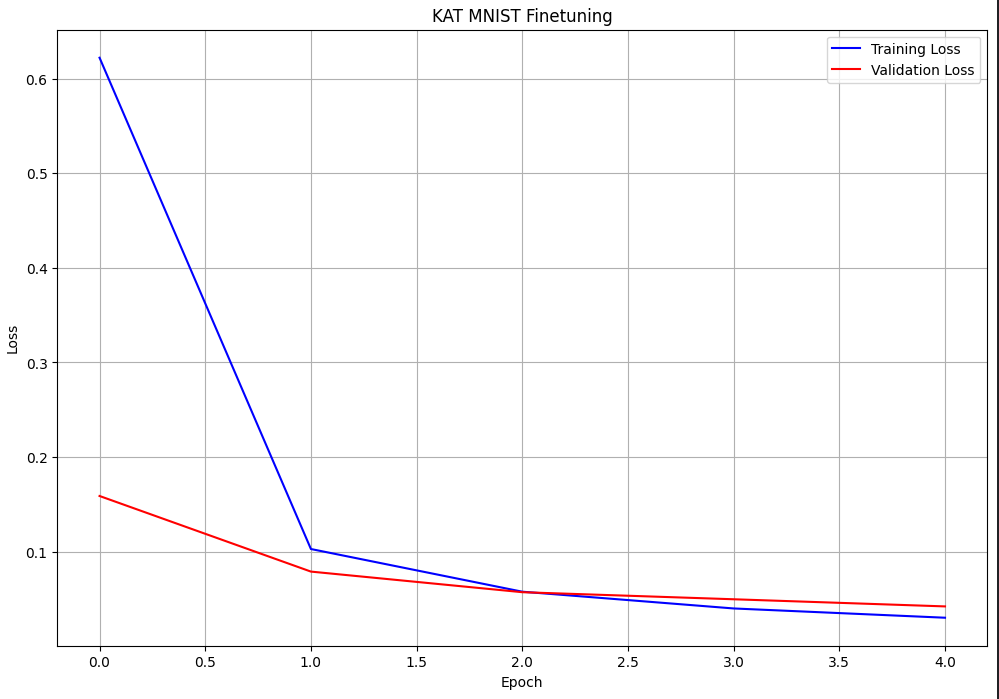
\includegraphics[width=0.65\linewidth]{mnist_train_val_loss.png}
    \caption{MNIST: Training (blue) vs.\ Validation (red) Loss.}
    \label{fig:mnist_loss}
\end{figure}

\begin{table}[H]
    \centering
    \scriptsize
    \begin{tabular}{lcccc}
        \toprule
        \textbf{Class}    & \textbf{Precision}          & \textbf{Recall} & \textbf{F1-score} & \textbf{Support} \\
        \midrule
        0                 & 0.99                        & 1.00            & 0.99              & 980              \\
        1                 & 0.99                        & 1.00            & 1.00              & 1135             \\
        2                 & 0.98                        & 1.00            & 0.99              & 1032             \\
        \ldots            & \ldots                      & \ldots          & \ldots            & \ldots           \\
        8                 & 0.99                        & 0.99            & 0.99              & 974              \\
        9                 & 0.99                        & 0.98            & 0.98              & 1009             \\
        \midrule
        \textbf{Accuracy} & \multicolumn{4}{c}{99.00\%}                                                          \\
        \bottomrule
    \end{tabular}
    \caption{MNIST Classification Report (partial).}
    \label{tab:mnist_report}
\end{table}

\subsection{FashionMNIST Finetuning Results}
FashionMNIST contains grayscale images of clothing items (10 classes) with an
original size of $28\times28$ \cite{fashionmnist}. The same preprocessing as
MNIST is applied.

Finetuning was also performed for 5 epochs using the AdamW optimizer in
conjunction with an early stopping mechanism, ultimately achieving a final test
accuracy of around 92.78\%. 

\begin{figure}[H]
    \centering
    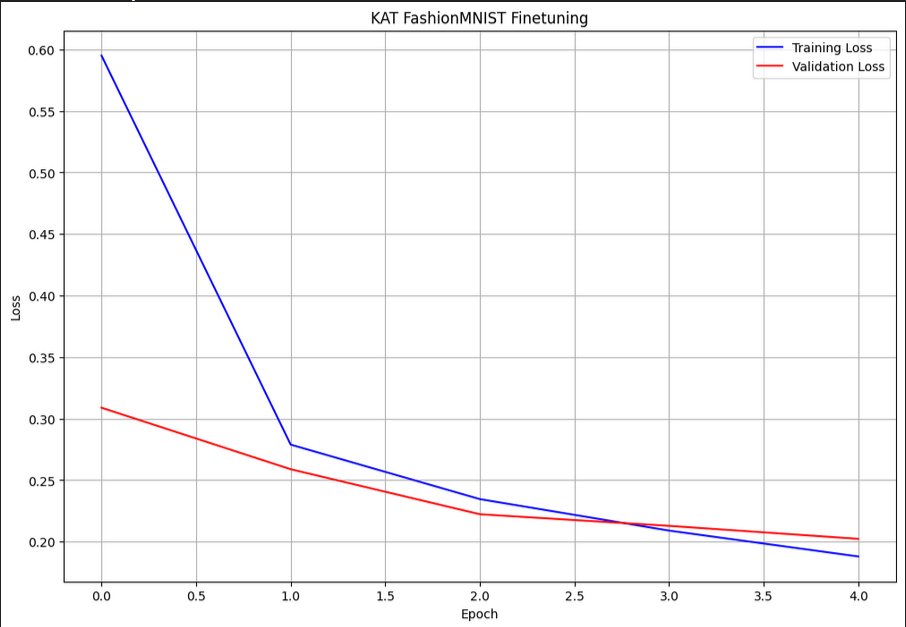
\includegraphics[width=0.55\linewidth]{fashionmnist_train_loss.png}
    \caption{FashionMNIST: Training vs.\ Validation Loss over 5 epochs.}
    \label{fig:fashionmnist_loss}
\end{figure}

\begin{table}[H]
    \centering
    \scriptsize
    \begin{tabular}{lcccc}
        \toprule
        \textbf{Class}    & \textbf{Precision}          & \textbf{Recall} & \textbf{F1-score} & \textbf{Support} \\
        \midrule
        0 (T-shirt/Top)   & 0.90                        & 0.85            & 0.87              & 1000             \\
        1 (Trouser)       & 0.99                        & 0.99            & 0.99              & 1000             \\
        2 (Pullover)      & 0.93                        & 0.87            & 0.90              & 1000             \\
        3 (Dress)         & 0.91                        & 0.92            & 0.92              & 1000             \\
        4 (Coat)          & 0.89                        & 0.93            & 0.91              & 1000             \\
        5 (Sandal)        & 0.99                        & 0.98            & 0.99              & 1000             \\
        6 (Shirt)         & 0.75                        & 0.82            & 0.79              & 1000             \\
        7 (Sneaker)       & 0.98                        & 0.95            & 0.96              & 1000             \\
        8 (Bag)           & 0.99                        & 0.99            & 0.99              & 1000             \\
        9 (Ankle Boot)    & 0.95                        & 0.98            & 0.97              & 1000             \\
        \midrule
        \textbf{Accuracy} & \multicolumn{4}{c}{93.01\%}                                                          \\
        \bottomrule
    \end{tabular}
    \caption{FashionMNIST Classification Report.}
    \label{tab:fashionmnist_report}
\end{table}

\subsection{CIFAR-10 Finetuning Results}
CIFAR-10 consists of 10 classes of color images (originally $32\times32$) which
are resized to $224\times224$ \cite{cifar}. Preprocessing involves
normalization with ImageNet statistics.

Similarly, for CIFAR-100, the model was finetuned
over 5 epochs with early stopping—where the best validation loss was recorded
at epoch 5—and a final test accuracy of approximately 95.70\% was obtained.

\begin{figure}[H]
    \centering
    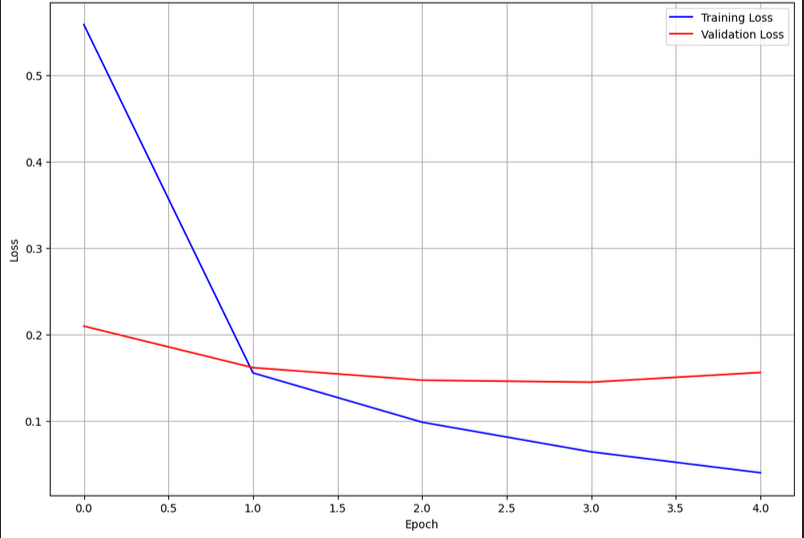
\includegraphics[width=0.55\linewidth]{cifar10_train_val_loss.png}
    \caption{CIFAR-10: Training vs.\ Validation Loss.}
    \label{fig:cifar10_loss}
\end{figure}

\begin{table}[H]
    \centering
    \scriptsize
    \begin{tabular}{lcccc}
        \toprule
        \textbf{Class}    & \textbf{Precision}          & \textbf{Recall} & \textbf{F1-score} & \textbf{Support} \\
        \midrule
        0 (Airplane)      & 0.98                        & 0.95            & 0.97              & 1000             \\
        1 (Automobile)    & 0.97                        & 0.98            & 0.97              & 1000             \\
        2 (Bird)          & 0.98                        & 0.95            & 0.97              & 1000             \\
        \ldots            & \ldots                      & \ldots          & \ldots            & \ldots           \\
        8 (Ship)          & 0.96                        & 0.99            & 0.98              & 1000             \\
        9 (Truck)         & 0.97                        & 0.96            & 0.97              & 1000             \\
        \midrule
        \textbf{Accuracy} & \multicolumn{4}{c}{95.70\%}                                                          \\
        \bottomrule
    \end{tabular}
    \caption{CIFAR-10 Classification Report (partial).}
    \label{tab:cifar10_report}
\end{table}

\subsection{CIFAR-100 Finetuning Results}
CIFAR-100 features 100 classes of color images (originally $32\times32$)
\cite{cifar} and is similarly preprocessed by resizing to $224\times224$ and
normalizing with ImageNet statistics.

Similarly, for CIFAR-100, the model was finetuned
over 5 epochs with early stopping—where the best validation loss was recorded
at epoch 5—and a final test accuracy of approximately 81.17\% was obtained.

\begin{figure}[H]
    \centering
    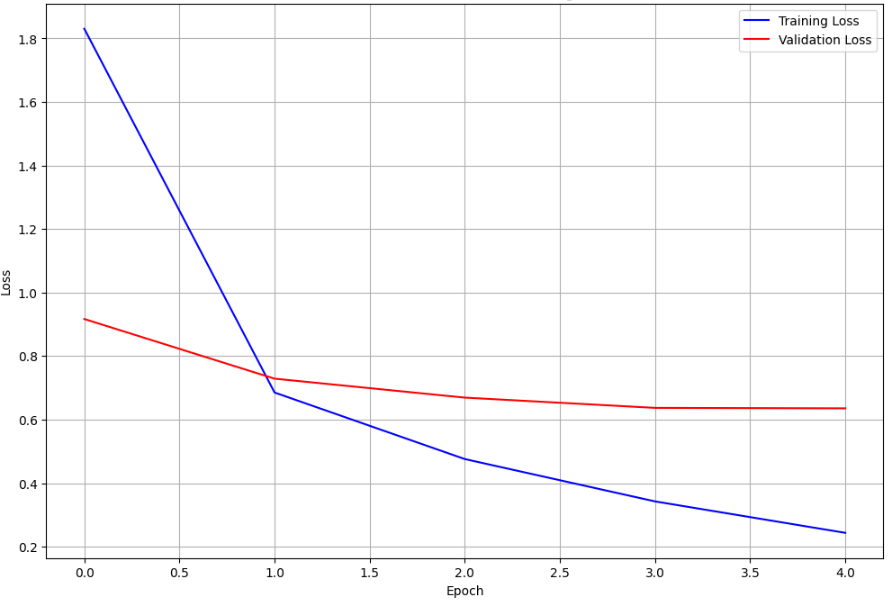
\includegraphics[width=0.55\linewidth]{cifar100_train_val_loss.png}
    \caption{CIFAR-100: Training vs.\ Validation Loss.}
    \label{fig:cifar100_loss}
\end{figure}

\begin{table}[H]
    \centering
    \scriptsize
    \begin{tabular}{lcccc}
        \toprule
        \textbf{Class}        & \textbf{Precision} & \textbf{Recall} & \textbf{F1-score} & \textbf{Support} \\
        \midrule
        Class 0               & 0.90               & 0.97            & 0.93              & 1000             \\
        Class 13              & 0.80               & 0.81            & 0.81              & 1000             \\
        Class 35              & 0.48               & 0.62            & 0.54              & 1000             \\
        \ldots                & \ldots             & \ldots          & \ldots            & \ldots           \\
        \midrule
        \textbf{Weighted Avg} & 0.82               & 0.81            & 0.81              & 10000            \\
        \bottomrule
    \end{tabular}
    \caption{CIFAR-100 Classification Report (excerpt).}
    \label{tab:cifar100_report}
\end{table}

\subsection{Summary of Finetuning Results}

Across all datasets, the finetuning procedure demonstrates that the pretrained
KAT model adapts efficiently to new tasks. Specifically, we achieved test
accuracies of approximately 99.00\% on MNIST, 93.01\% on FashionMNIST, 95.70\%
on CIFAR-10, and 81.17\% on CIFAR-100. These results highlight the versatility
of the KAT architecture, which effectively leverages large-scale pretrained
features and GPU parallelism to achieve strong performance on diverse image
recognition tasks within a short finetuning period. Moreover, the KAT model
effectively and efficiently retains the previously learned knowledge from
pretraining, adjusting quickly and properly to new information. Overall, our
results demonstrate the potential of KAT models for image recognition tasks and
the benefits of leveraging such pretrained models for efficient transfer
learning.

\bibliography{bib}
\bibliographystyle{plainnat}

\end{document}



